\section*{Frequency Analysis}
\addcontentsline{toc}{section}{Frequency Analysis}
The first part of this assignment is to establish the frequencies of the letters
$[A \dots Z]$ of the British language. To do that I created the
FrequencyAnalyzer.java class, that uses regex\cite{Regex} to remove anything
but the $[A \dots Z]$ letters, and then counts the number of each in the text. 
The text I chose as a representation of british-english is: Pride and Prejudice
by Jane Austen, taken from Project Gutenberg\cite{PnP}.
\section*{Decryption Tool}
\addcontentsline{toc}{section}{Decryption Tool}
To help with decrypting text I have developed a small decryption tool. This tool
takes a file as input, and selects a line of text from that file at random, this
is then encrypted using a substitution cipher. The cipher is generated anew by
the tool each time a new cryptogram is displayed.
\FloatBarrier
\begin{figure}[h]
\centering
\makebox[\textwidth]{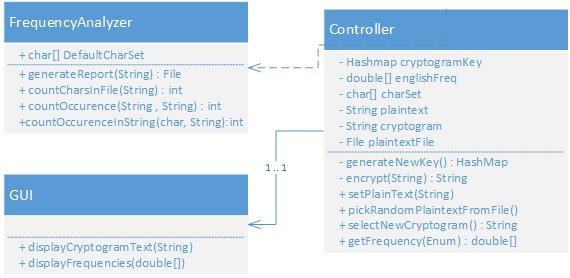
\includegraphics[width=\textwidth]{project1_ClassDiag}}
\caption{\emph{Class Diagram}: Only the most relevant methods and class
variables have been displayed.}
\label{fig:ClassDia}
\end{figure}
\FloatBarrier
\subsection*{Controller}
\addcontentsline{toc}{subsection}{Controller}
The controller class Is responsible for managing any data in the program, and
responds to requests from the GUI.
\subsection*{GUI}
\addcontentsline{toc}{subsection}{GUI}
The gui manages the look and feel of the program, It also handles key-events,
such as updating all coresponding frames when a letter is chose for the
cryptogram, and action-events such as buttons.
\subsection*{FrequencyAnalyzer}
\addcontentsline{toc}{subsection}{FrequencyAnalyzer}
The frequencyAnalyzer is a static helper class, it is only used to calculate the
frequencies of the cryptogram, It's other functions as described in the
section Frequency Analysis, are used seperately.
\section*{Conclusion}
\addcontentsline{toc}{section}{Conclusion}
My tool can display a plaintext, give hints, display frequencies for both
english and the cryptogram, select a new cryptogram from a given list, and solve
the cryptogram if asked.\\
However it solves by simply giving the solution, as I did not have the
time to implement chi-square test, and it has no support for n-grams in the
cryptogram, as I only managed to partly implement this before having to move on
to Program2.
